\chapter{PELAKSANAAN PENELITIAN}
\label{pelaksanaan-penelitian}

\section{Alat dan Bahan Penelitian}
Penelitian ini tidak dapat dilakukan tanpa adanya alat dan bahan yang memudahkan penulis dalam melakukan penelitian. Alat dan bahan yang digunakan oleh penulis disebutkan secara rinci pada Tabel \ref{tbl:4:alatbahan}, dan Tabel \ref{tbl:4:speklaptop}.

\vspace{2em}
\begin{table}[!h]
	\caption{Daftar alat dan bahan}
	\label{tbl:4:alatbahan}
	\centering
	% use packages: array
	\begin{tabular}{|c|p{3.6cm}|p{9cm}|}
		\hline
		No. & Nama alat/bahan & Fungsi \\
		\hline
		1 & ASUS N550JX & Perangkat komputer \\ \hline
		2 & IES-VE 2019 & Perangkat lunak untuk pengambilan data lingkungan termal \textit{climate chamber} dan variasi gangguan \\ \hline
		3 & MS Excel 365 & Perangkat lunak pengolahan data tabular \\ \hline
		4 & MATLAB R2018a & Perangkat lunak pemrograman dalam merancang jaringan saraf tiruan dan sistem kontrol. \\ \hline
		5 & Simulink & Perangkat lunak untuk menjalankan simulasi sistem kontrol. \\ \hline
		%5 & VS Code 1.38 & Aplikasi penulisan dan penyuntingan kode sumber \\ \hline
		%6 & Python 3.7 & Bahasa pemrograman \\ \hline
		%7 & Anaconda 3 & Distribusi pengelola lingkungan pengembangan dan manajemen paket untuk komputasi ilmiah \\ \hline
		%8 & Jupyter Notebook 1.0 & Aplikasi web untuk menulis kode program, teks, persamaan, dan visualisasi \\ \hline
		%9 & Pandas 1.0.3 & Pustaka manupulasi dan analisis data \\ \hline
		%10 & Scikit-Learn 0.21 & Pustaka pembangunan \textit{Machine Learning} \\ \hline
		%11 & fireTS 0.0.7 & Pustaka prediksi deret waktu multivarian \\ \hline
		%6 & Raspberry Pi versi 3 B & Komputer mikro sebagai perangkat pengendali. \\ \hline
	\end{tabular}
\end{table}

\vspace{2em}
\begin{table}[!h]
	\caption{Spesifikasi laptop ASUS N550JX}
	\label{tbl:4:speklaptop}
	\centering
	% use packages: array
	\begin{tabular}{|c|p{5cm}|p{8cm}|}
		\hline
		No. & Komponen & Spesifikasi \\ \hline
		1 & Processor & Intel Core i7-4720HQ CPU @ 2.60GHz x 8 \\ \hline
		2 & Graphics & Intel Haswell Mobile \\ \hline
		3 & RAM & 8 GB \\ \hline
		4 & Tipe sistem operasi & 64-bit \\ \hline
		5 & Sistem operasi & Windows 10 Home Single Language \\ \hline
		%6 & Sistem operasi & Manjaro Linux \\ \hline
	\end{tabular}
\end{table}

\vspace{2em}
\section{Tata Laksana Penelitian}
Alur penelitian yang digunakan penulis dalam mencapai tujuan dapat dilihat pada Gambar \ref{fig:4:TataLaksanaPenelitian} berikut.
\begin{figure}[!b]
	\centering
	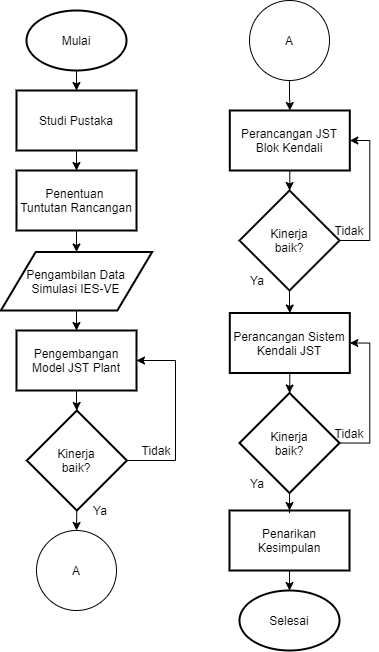
\includegraphics[width=0.7\textwidth]{figures/TataLaksanaPenelitian}
	\caption{Bagan Tata Laksana Penelitian}
	\label{fig:4:TataLaksanaPenelitian}
\end{figure}

%\begin{figure}[!h]
%	\centering
%	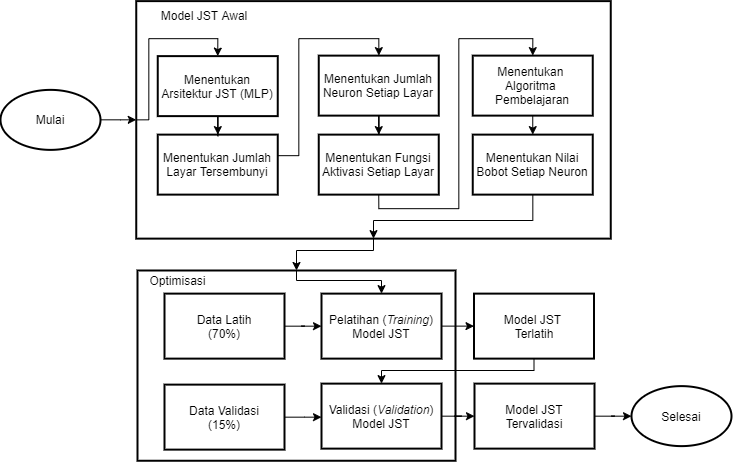
\includegraphics[width=0.85\textwidth]{figures/PerancanganModel}
%	\caption{Bagan Perancangan Model JST}
%	\label{fig:4:DiagramPerancanganModel}
%\end{figure}

%\begin{landscape}
%	\begin{figure}[!h]
%		\centering
%		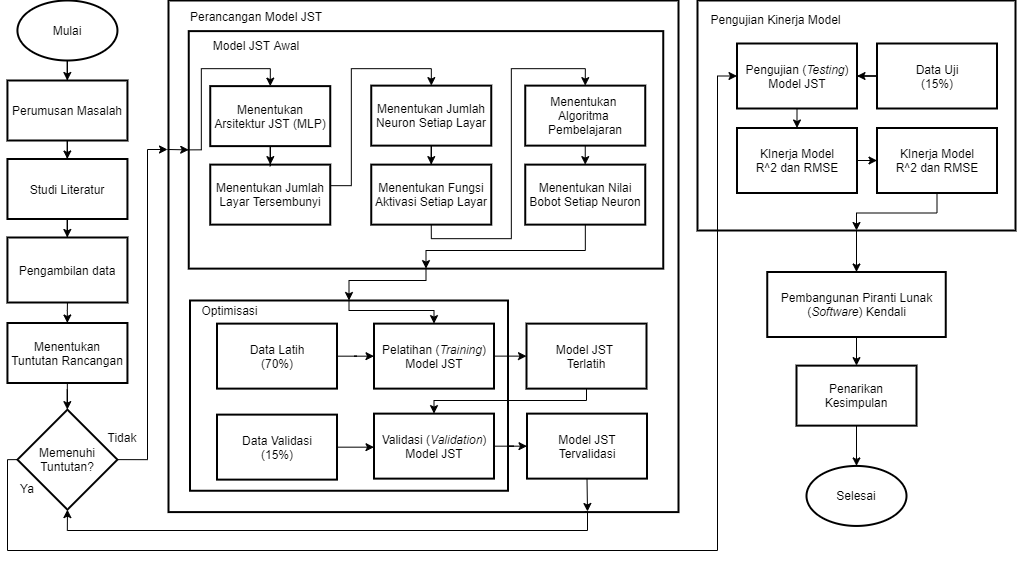
\includegraphics[width=1.5\textwidth]{figures/DiagramPenelitianFull}
%		\caption{Diagram Alir Penelitian Utuh}
%		\label{fig:4:DiagramPenelitianFull}
%	\end{figure}
%\end{landscape}

\subsection{Studi Pustaka}
Studi pustaka bertujuan untuk mendapatkan pemahaman dalam penyelesaian masalah yang diangkat dalam penelitian ini. Studi pustaka juga membantu menegaskan tujuan penelitian sehingga penulis mampu mengetahui perbedaan penelitian ini dengan penelitian terkait yang telah dilakukan sebelumnya. Dari studi pustaka yang telah dilakukan maka akan memperjelas tuntutan perancangan dari sistem yang akan dibuat. Informasi yang digunakan bersumber dari berbagai artikel ilmiah, jurnal, skripsi, buku, dan/atau sumber tertulis lainnya yang membahas mrengenai sistem kontrol lingkungan termal dan/atau jaringan saraf tiruan.

\subsection{Penentuan Tuntutan Rancangan}

Penulis dituntut untuk mampu membangun sistem kendali yang mampu mengendalikan \textit{plant} sesuai dengan \textit{setpoint} yang diinginkan mengikuti skema pengujian pada penggunaan \textit{climate chamber}.

\subsection{Pengambilan Data Simulasi IES-VE}
Penelitian ini menggunakan data yang sama dengan data yang digunakan oleh penelitian Tanto \cite{skripsiTanto} yang bersumber dari model yang telah dibuat di penelitian sebelumnya berjudul "Karakterisasi Lingkungan Termal Chamber Iklim Menggunakan Metode Simulasi CFD dengan Perangkat Lunak IES-VE" yang diteliti oleh Ichfan Kurniawan \cite{skripsiIchfan}.  Data tersebut merupakan hasil simulasi pada \textit{software} IES-VE dengan menerapkan beberapa variasi kondisi lingkungan pada model \textit{climate chamber}. Variasi tersebut yaitu kondisi batas lingkungan (radiasi matahari dan suhu bola kering luar / \textit{outdoor dry bulb temperature}), kondisi AC, dan kondisi \textit{heater}. Variasi kondisi batas lingkungan tersebut diwujudkan dalam pembagian 4 musim dalam 1 tahun, yakni bulan maret, juni, september dan desember. Keluaran dari model IES-VE berupa nilai suhu udara ruang (\textit{air temperature}) \textit{chamber} dan kelembapan relatif (RH) \textit{chamber}. Dari model tersebut didapatkan nilai MAE perhitungan selisih variabel lingkungan termal hasil simulasi dan pengukuran lapangan sebesar 0,8 $\pm$ 0,7$^{\circ}$C untuk suhu udara ruang dan 2,5 $\pm$ 3,8\% untuk kelembaban relatif \cite{skripsiIchfan}. Data yang sudah terkumpul disajikan dalam bentuk tabular yang kemudian diolah dalam program komputer yang dibuat oleh penulis.

\subsection{Pengembangan Model Plant JST}
Penelitian ini menggunakan model \textit{plant} yang telah dirancang dari penelitian sebelumnya berjudul "Pemodelan Lingkungan Termal Sistem \textit{Climate Chamber} dengan Metode Jaringan Saraf Tiruan" yang diteliti oleh Tri Hartanto \cite{skripsiTanto}. Model tersebut merupakan hasil perancangan pada piranti lunak MATLAB. Model \textit{plant} tersebut memiliki nilai MAE perhitungan antara target dan prediksi sebesar 0,59$^{\circ}$C untuk suhu udara ruang dan 5,44\% untuk kelembapan relatif. Akurasi JST sebesar 96,23\% untuk suhu udara ruang dan 68,90\% untuk kelembapan relatif \cite{skripsiTanto}. Model \textit{plant} ini akan digunakan oleh penulis dalam melakukan perancangan sistem kontrol berbasi jaringan saraf tiruan. Arsitektur Model Plant JST dijabarkan oleh Gambar \ref{fig:4:NNPlantModelDesign} di bawah ini.

\begin{figure}[!h]
	\centering
	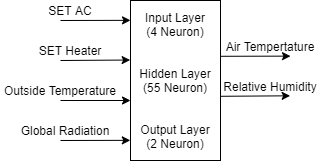
\includegraphics[width=0.65\textwidth]{figures/NNPlantModelDesign}
	\caption{Arsitektur Model Plant JST}
	\label{fig:4:NNPlantModelDesign}
\end{figure}

\subsection{Perancangan Sistem kontrol JST}
Perancangan sistem kontrol JST untuk lingkungan termal \textit{climate chamber} menggunakan diagram blok \textit{Neural Network Internal Model Control} (NN-IMC).Diagram blok tersebut dijabarkan pada Gambar \ref{fig:4:ConstrolSystemBlockDiagram} dibawah ini:

\begin{figure}[!h]
	\centering
	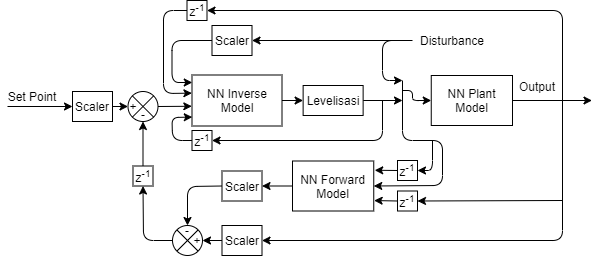
\includegraphics[width=0.9\textwidth]{figures/ControlDesignDiagram}
	\caption{Blok Diagram Sistem Kendali JST}
	\label{fig:4:ConstrolSystemBlockDiagram}
\end{figure}

\begin{figure}[!b]
	\centering
	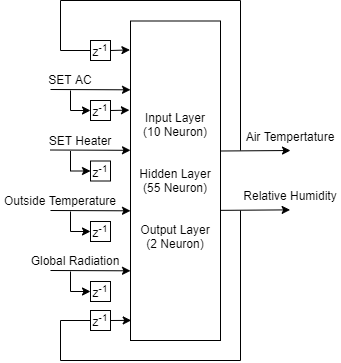
\includegraphics[width=0.5\textwidth]{figures/NNForwardModelDesign}
	\caption{Arsitektur NN Forward Model}
	\label{fig:4:NNForwardModelDesign}
\end{figure}

\begin{figure}[!t]
	\centering
	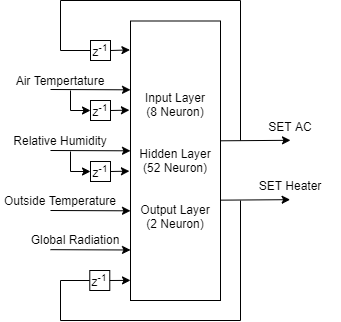
\includegraphics[width=0.5\textwidth]{figures/NNInverseModelDesign}
	\caption{Arsitektur NN Inverse Model}
	\label{fig:4:NNInverseModelDesign}
\end{figure}

Pada Gambar diatas, Penulis menggunakan Model Invers JST (NN Inverse Model) dari Plant sebagai kontroler dan Model Umpan JST (NN Forward Model) sebagai emulator.

Perancangan JST untuk kontroler menggunakan output plant, disturbance, delay umpan balik dan delay output plant sebagai sebagai input sebagai untuk pelatihan JST. NN Inverse Model dijelaskan pada Gambar \ref{fig:4:NNInverseModelDesign} dan NN Forward Model dijelaskan pada Gambar \ref{fig:4:NNForwardModelDesign}.\\

\subsection{{Penarikan Kesimpulan}}
Penarikan kesimpulan didapatkan berdasarkan hasil model terbaik yang terpilih dari beberapa percobaan variasi penentuan jumlah \textit{hidden layer} dan/atau jumlah neuron untuk kontroler JST serta berbagai percobaan diagram blok sistem kontrol. Kesimpulan menggambarkan bagaimana parameter model yang terpilih dan rancangan diagram blok sistem kontrol sehingga dapat digunakan sebagai sistem kontrol lingkungan termal pada \textit{climate chamber} DTNTF FT UGM.

\section{Rencana Analisis Hasil Penelitian}
Terdapat 3 objek yang akan dianalisis oleh penulis, yaitu model plant JST, kontroler JST, dan Sistem Kontrol JST. Kinerja dari model plant JST akan dievaluasi berdasarkan nilai MAE (\textit{Mean Absolute Error}) dan R (koefisien korelasi) dibandingkan dengan rancangan penelitian sebelumnya. Kinerja dari kontroler  JST akan dievaluasi berdasarkan nilai MSE (\textit{Mean Squared Error}) dan R (koefisien korelasi) dari rancangan JST tersebut. Kinerja dari sistem kontrol akan dievaluasi berdasarkan nilai Kesalahan Keadaan Ajeg.